\documentclass{IEEEtran}
\usepackage{color}
\usepackage{array}
\usepackage{float}
\usepackage{amsmath}
\usepackage{amssymb}
\usepackage{graphicx}
\usepackage{algorithm}
\usepackage{algorithmic}
\usepackage{paralist}
\usepackage{cite}
 \usepackage{color}
\usepackage{amsfonts}
\usepackage{mathtools}
\usepackage{multirow}
\usepackage{subfigure}
\usepackage{tikz}
\usepackage{pgf}
\usepackage{pgfplots}
\usepackage{url}
\DeclareGraphicsExtensions{.pdf,.png,.jpg,.eps}

\begin{document}
\title{Acceleration of Bilateral filtering algorithm for manycore and multicore architectures}
\author{\IEEEauthorblockN{Dinesh Agarwal, Sami Wilf, Abinashi Dhungel, and Sushil K. Prasad}\\
\IEEEauthorblockA{ Georgia State University\\
 Department of Computer Science\\
 Atlanta, Georgia 30303\\
 }}
\maketitle
\begin{abstract}
This work explores multicore and manycore acceleration for the embarrassingly parallel, compute-intensive Bilateral filtering kernel. For manycore architectures, we have created a pair-symmetric algorithm to avoid redundant calculations and for multicore architectures we improve the algorithm by use of low level single instruction multiple data (SIMD) parallelism across multiple threads. We present empirical data evidencing the performance gains we achieved over variety of hardware architectures including Nvidia GTX280, AMD Barcelona, AMD Shanghai, Intel Harpertown, AMD Phenom, Intel Core i7 quad core, and Intel Nehalem 32 core machines. The best speedup achieved was a 235.5x speedup by our CUDA-based implementation of our pair-symmetric algorithm running on Nvidia's GTX280. Our CPU multicore implementations resulted in a speedup of up to 38x using 16 cores of AMD Barcelona each with 4-stage vector pipeline, up to 23x using 8 cores for Intel Harpertown, and up to 26x using 32 cores of Intel Nehalem multicore machines compared to a compiler-optimized code.
\end{abstract}
% For peer review papers, you can put extra information on the cover
% page as needed:
% \ifCLASSOPTIONpeerreview
% \begin{center} \bfseries EDICS Category: 3-BBND \end{center}
% \fi
% For peerreview papers, this IEEEtran command inserts a page break and
% creates the second title. It will be ignored for other modes.
\IEEEpeerreviewmaketitle
\section{Introduction}
\label{sec:intro} The recent advances in parallel computing and architecture design have provided a series of avenues for application performance improvements. However, unlike the days when applications automatically became faster with increased clock frequency, newer chips require programmers and researchers to revisit their algorithm designs to harness the power of underlying architectures. Moreover, there is no well defined list of guidelines that can be followed for each application, which makes it challenging to deploy existing applications, even fundamental ones, to a myriad of available multicore and manycore architectures.

Our work explores efficient parallel implementation of Bilateral filtering kernel\footnotemark[1] proposed by Tomasi and Manduchi \cite{Tomasi1998}, on multicore and manycore architectures. Bilateral filtering kernel is used to smooth an image without blurring its edges. It is ubiquitous in various image processing applications in various contexts such as denoising\cite{zhang2008}, texture editing and relighting\cite{eisemann2004}, tone management\cite{Bae2006}, stylization\cite{DeCarlo2002}, optical-flow estimations\cite{Xiao2006}, and demosaicking\cite{Ramanath2003} etc. 

A faster approximation to the original algorithm \cite{Paris2009} extends the image to 3D space by treating the pixel intensity as the third dimension and using a linear shift-invariant convolution in 3D. A separable implementation \cite{Pham2005} applies the filter kernel first to one of the image dimensions and the intermediate result is filtered again on other dimensions. This reduces the complexity from $O(N*(m^{d}))$ to $O(N*d)$, where $N$ is the total number of pixels in the image and $d$ is the dimensions of the image. Yang et al.\cite{yang2009} have reported a constant time algorithm by dividing the Bilateral filtering kernel into a constant number of time spatial kernels. However, we do not parallelize these methods since our interest is to develop a parallelization method that can be applied, in general, to any spatially invariant and inseparable filtering algorithm. 

In this paper, we propose a set of optimizations and a non-naive algorithm for Bilateral filtering kernel. Specifically, we introduce a pair-symmetric algorithm which has the theoretical potential to reduce processing time to half. We propose architecture specific optimizations, such as exploiting the unique capabilities of special registers available in modern multicore architectures and the rearrangement of data access patterns as per the computations to exploit special purpose instructions. We also propose optimizations pertinent to Nvidia's CUDA, including utilization of CUDA's implicit synchronization capability and the maximization of single-instruction-multiple-thread efficiency. 

In order to assess the efficacy of our optimization techniques, our experimental testbed includes a comprehensive set of multicore and manycore architecture chips including the Nvidia GTX280, AMD quad-core 2376 (Shanghai), AMD quad-core 8350 (Barcelona), Intel quad-core Xeon E5410 (Harpertown), Intel eight-core Xeon X7560 (Nehalem-EX), Intel quad-core Core i7, and AMD Phenom II six-core architectures. \footnotetext[1]{Our code is available under GNU GPL license from \url{http://code.google.com/p/blfilter/}.}

Rest of the paper is organized as following: Section~\ref{sec:stencil} defines the Bilateral filtering kernel and introduces a naive algorithm and our pair-symmetric algorithm for Bilateral filtering. Section~\ref{sec:GPUoptimizations} introduces the optimizations employed to devise the pair-symmetric algorithm for CUDA architectures. Section~\ref{sec:optimizations} introduces the optimizations for CPU architectures and establishes the rationale behind ignoring traditional memory related optimizations for Bilateral filtering kernel. Our hardware and software testbed for experiments is detailed in Section~\ref{sec:expt}, immediately followed by Section~\ref{sec:results} that reports the performance of Bilateral filtering kernel on both multicore and manycore architectures. Section~\ref{sec:conclusion} concludes this paper with remarks on general applicability of our optimizations.

\section{Bilateral Filtering Kernel}
\label{sec:stencil} 

\begin{figure}[h!]
\centering 
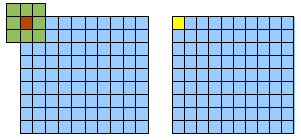
\includegraphics[width=3.2in]{images/filter} 
\caption{Example of a filter at the starting position of the image}
\label{fig:filter} 
\end{figure}

Filtering, an essential application of image processing, is carried out by a relatively small window, known as the filter (``Filter'' or ``Window''), which iterates over the source image, performing the same execution at each step of the iteration. The elements that the Filters cover in a given iteration makeup the neighborhood (``Neighborhood'') and are neighbors (``Neighbors'' or ``Neighboring Pixels'') of the Filter's center element (``Center'' or ``Center Pixel''). 

Figure~\ref{fig:filter} illustrates the starting position of the Filter as commonly seen in standard, image processing algorithms; the source image is on the left and the destination image on the right is used to store the result of the Filter's computation at the respective Center's position.

Bilateral filtering combines two different kernels - the spatial kernel and the photometric kernel. With the photometric kernel, when the Center of the Filter rests on a pixel that boarders or is a part of a pictorial edge, e.g., an outline of an object or person against a contrasting background, the Neighbors that make up the other (contrasting) side of the edge have an insignificant impact on the Center Pixel's corresponding output pixel, which is stored in the destination array storing the processed image. Furthermore, when the Center is not bordering, and is not a part of a pictorial edge, the Neighbors contribute equally and the noise is filtered out. Hence, pictorial edges maintain sharpness while noise in the pictorial regions are filtered, resulting in more appealing images. Mathematically, the Bilateral filter can be defined in terms of the spatial kernel and photometric kernel as follows\cite{Tomasi1998}:\\

Spatial kernel: 
\begin{equation}
h(x)=k_{d}^{-1}(x)\int_{-\infty}^{\infty}\int_{-\infty}^{\infty}f(\xi)c(\xi,x)d\xi\label{spatial}
\end{equation}
 
\begin{equation}
k_{d}(x)=\int_{-\infty}^{\infty}\int_{-\infty}^{\infty}c(\xi,x)d\xi
\end{equation}
 Photometric kernel: 
\begin{equation}
h(x)=k_{r}^{-1}(x)\int_{-\infty}^{\infty}\int_{-\infty}^{\infty}f(\xi)s(f(\xi),f(x))d\xi\label{photometric}
\end{equation}
 
\begin{equation}
k_{r}(x)=\int_{-\infty}^{\infty}\int_{-\infty}^{\infty}s(f(\xi),f(x))d\xi
\end{equation}


The combined kernel, which is the Bilateral filter, is the product
of spatial kernel and photometric kernel and is described as: 
\begin{equation}
h(x)=k^{-1}(x)\int_{-\infty}^{\infty}\int_{-\infty}^{\infty}f(\xi)c(\xi,x)s(f(\xi),f(x))d\xi\label{combined}
\end{equation}
 
\begin{equation}
k(x)=\int_{-\infty}^{\infty}\int_{-\infty}^{\infty}c(\xi,x)s(f(\xi),f(x))d\xi
\end{equation}

Function $c(\xi,x)$ measures the $geometric~closeness$ between neighborhood Center $x$ and a Neighbor $\xi$. Function $s(f(\xi),f(x))$ measures the $photometric$ $similarity$ (similarity in pixel intensity) between the same. The influence of a Neighbor on the Filter's output computation, for a Center Pixel, is calculated as a product of spatial kernel and the photometric kernel. Thus, Neighbors with similar photometric properties influence the Center Pixel more than those with less similar photometric properties. This results in edge-preserved image smoothing, which is the purpose of the Bilateral filter. It should be noted, however, that the foregoing equations are mathematical representations for filtering of infinite-precision images. As infinite-precision is a concept more pertinent to the analog domain and does not exist in the digital domain, each double integral in equations 1-6 must be understood as the summation of a finite set of calculations, i.e. one calculation per Neighbor and one set of calculations per Center Pixel, or put another way, one set of calculations per Filter iteration. A formal expression is given below:

\begin{equation}
\label{eq:depen}
filtered\: pixel\: x=\frac{\substack{N\\
\sum\\
i=1
}
f(\xi_{i})\cdot c(\xi_{i},x)\cdot s(f(\xi_{i}),f(x))}{\substack{N\\
\sum\\
i=1
}
c(\xi_{i},x)\cdot s(f(\xi_{i}),f(x))}
\end{equation}

In addition to restating the Bilateral filter's mathematical model in terms of a finite summation, Equation~\ref{eq:depen} reveals the data dependency that exists in the Bilateral filter. Specifically, Equation~\ref{eq:depen} shows that before the filtered pixel can be calculated by dividing the numerator by the denominator, both the summation in the numerator and denominator must first be calculated. Consequently, the Bilateral filter has two data dependencies. As explained later in this paper, the pair-symmetric algorithm significantly increases the memory consumption in order to manage data dependencies but pays off by cutting, in half, the total number of executions.

Another observation taken into account is that the values of Equation~\ref{spatial}, for the Neighborhood, can be computed in advance as the values depend on a simple Gaussian probability distribution function. However, the values of Equation~\ref{photometric} and consequently of Equation~\ref{combined} cannot be known a priori as they depend on the similarity of signals between the current Center Pixel and the Neighborhood. Moreover, as the size of the Window increases, which only happens by choice of the user as the size is user defined, the number of computations per pixel grows at a rate of $O(FilterWindowWidth^{2})$ where FilterWindowWidth is the diameter of the Window. By reason of the foregoing, the bulk of the time spent in processing an image using the Bilateral filter is in the arithmetic-intensive computations, because the number of writes to the destination image is constant as the rate of growth of Center-Neighbor computations with respect to the Window size increase.

\subsection{A Naive Approach to Bilateral filtering kernel}

\begin{figure}
\centering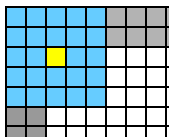
\includegraphics[scale=0.35]{images/the1}
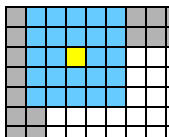
\includegraphics[clip,scale=0.35]{images/the202}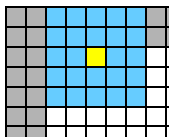
\includegraphics[scale=0.35]{images/the2}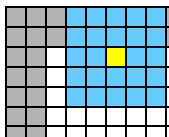
\includegraphics[scale=0.35]{images/the3}
\caption{Example of a naive Bilateral filter iterations}
\end{figure}

The naive stencil algorithm is the standard model that is predominantly used in Bilateral filtering kernel. Previous implementations\cite{Paris2009,Pham2005} of Bilateral filtering kernel improves the hardware dependent aspects and hence expend resources on achieving performance gains that can not match the effort taken. Here, we address a root problem of the standard naive algorithm by proposing a new algorithm, and then develop hardware dependent improvements for further speedup. Algorithm~\ref{alg:Example-Algorithm-float} is the pseudo-code for the standard naive Bilateral filtering kernel.

%\begin{algorithm}[!h]
%\caption{Generalized Naive Stencil Kernel Algorithm}
%\label{alg:Example-Algorithm-float}
%\begin{algorithmic}
%\FORALL{element  $s_{i,j}$ in source image s}
%\FORALL{data dependency $n$}
%\STATE{$X_n \leftarrow 0$}
%\ENDFOR
%\FOR{$k=-filter\_hw$ \TO $filter\_hw$}
%\FOR {$l  = -filter\_hw$ \TO $filter\_hw$}
%\FORALL{data dependency $n$}
%\STATE{$X_n \leftarrow X_n + f_n(s[i,j],s[i+k,j+l])$}
%\ENDFOR
%\ENDFOR
%\ENDFOR
%\STATE{output[$i,j] \leftarrow f_{output}(X_{1}, \dots, X_{last})$}
%\ENDFOR
%\end{algorithmic}
%\end{algorithm}

\begin{algorithm}[!h]
\caption{Naive Bilateral Filter Algorithm}
\label{alg:Example-Algorithm-float}
\begin{algorithmic}
\FORALL{element  $s_{i,j}$ in source image s}
\STATE{$X_{1} \leftarrow 0$}
\STATE{$X_{2} \leftarrow 0$}
\FOR{$k=-filter\_hw$ \TO $filter\_hw$}
\FOR {$l  = -filter\_hw$ \TO $filter\_hw$}
\STATE{$temp \leftarrow e^{C_1(k^2 + l^2) + C_2(s[i,j] - s[i,j+l])^{2}}$}
\STATE{$X_1 \leftarrow X_1 + temp \cdot s[i+k,j+l]$}
\STATE{$X_2 \leftarrow X_2 + temp$}
\ENDFOR
\ENDFOR
\STATE{output[$i,j] \leftarrow X_{1} / X_{2}$}
\ENDFOR
\end{algorithmic}
\end{algorithm}

\subsection{Pair-symmetric Bilateral filtering kernel}
The pair-symmetric algorithm, shown in Algorithm~\ref{alg:Example-Algorithm-float-1}, reduces the amount of Center-Neighbor computations by half. Thus, it can theoretically cut the processing time in half at the cost of increased memory requirement, which increases with the amount of dependencies. Its implementation is non-trivial due to potential race-conditions.
	
Our pair-symmetric Bilateral filtering algorithm is premised on the fact that each pixel assumes the role of both a Center Pixel and a Neighboring Pixel, and that the codes are symmetric with respect to Center-Neighbor paired computations. For example, in the Bilateral filter, $c(\xi,x)$ returns the same value as $c(x,\xi)$ and $s(f(\xi),f(x))$ returns the same value as $s(f(x),f(\xi))$. It then follows that the naive Bilateral filtering algorithm dictated in Algorithm~\ref{alg:Example-Algorithm-float} above, although simple, performs twice as many calculations than necessary.

The Pair-symmetric algorithm eliminates this redundancy that is inherent in the naive Bilateral filtering algorithm. Instead of reading from all Neighbors, our pair-symmetric algorithm reads from only half of the Neighbors. The result of each Center-Neighbor paired computation is then added to the $X_n$ register, which eventually obtains the result of data dependency $n$. This is trivial as the naive Bilateral filtering algorithm already does this. What our pair-symmetric algorithm does unique is that the result of each Center-Neighbor paired computation is also added to and stored in the Neighbor's position in a temporary array ("Map'') that is used for storing the results of a data dependency. So, there are $n$ Maps for $n$ number of dependencies. 

After the data dependency conditions are met, the function that returns the output data from the dependencies iterates over the Maps. As applied to the Bilateral filter, the data dependency lies in calculating each pixel's numerator and denominator that is used to derive the pixel's output result. After the numerators and denominators are derived, a function iterates and divides the corresponding elements of the two arrays to return the output. 

%\begin{algorithm}[h]
%\caption{Pair-symmetric Stencil Algorithm}
%\label{alg:Example-Algorithm-float-1}
%\begin{algorithmic}
%\STATE /* D is the set of dependency arrays */
%\FORALL{data dependency $n$}
%\FORALL{element $s_{i,j}$ in source image s}
%\STATE{$D_n[i,j] \leftarrow 0$}
%\ENDFOR
%\ENDFOR
%\FORALL{element $s_{i,j}$ in source image $s$}
%\FOR{$k=1$ \TO $filter\_hw$}
%\FOR{$l = -filter\_hw$ \TO $filter\_hw$}
%\FORALL{data dependency $n$}
%\STATE $temp \leftarrow f_n(s[i,j],s[i+k,j+l])$
%\STATE $D_n[i,j] \leftarrow D_n[i,j] + temp$
%\STATE $D_n[i+k,j+l] \leftarrow D_n[i+k,j+l] + temp$
%\ENDFOR
%\ENDFOR
%\ENDFOR
%\FOR{$l = -filter\_hw$ \TO $0$}
%\FORALL{data dependency $n$}
%\STATE $temp \leftarrow f_n(s[i,j],s[i,j+l])$
%\STATE $D_n[i,j] \leftarrow D_n[i,j] + temp$
%\STATE $D_n[i,j+l] \leftarrow D_n[i,j+l] + temp$
%\ENDFOR
%\ENDFOR
%\ENDFOR
%\FORALL{element $s_{i,j}$ in source image s}
%\STATE{$output[i,j] \leftarrow f_{output}(D_{1}[i,j], \dots, D_{last}[i,j])$}
%\ENDFOR
%\end{algorithmic}
%\end{algorithm}




%\begin{algorithm}[h]
%\caption{Pair-symmetric Bilateral Filtering kernel}
%\label{alg:Example-Algorithm-float-1}
%\begin{algorithmic}
%\STATE /* D is the set of dependency arrays */
%\FORALL{element $s_{i,j}$ in source image s}
%\STATE{$D_1[i,j] \leftarrow 0$}
%\STATE{$D_2[i,j] \leftarrow 0$}
%\ENDFOR
%\FORALL{element $s_{i,j}$ in source image $s$}
%\FOR{$k=1$ \TO $filter\_hw$}
%\FOR{$l = -filter\_hw$ \TO $filter\_hw$}
%\STATE{$temp \leftarrow e^{C_1(k^2 + l^2) + C_2(s[i,j] - s[i+k,j+l])^{2}}$}
%\STATE{$D_1[i,j] \leftarrow D_1[i,j] + temp \cdot s[i+k,j+l]$}
%\STATE{$D_2[i,j] \leftarrow D_2[i,j] + temp$}
%\STATE{$D_1[i+k,j+l] \leftarrow D_1[i+k,j+l] + temp \cdot s[i,j]$}
%\STATE{$D_2[i+k,j+l] \leftarrow D_2[i+k,j+l] + temp$}
%\ENDFOR
%\ENDFOR
%\FOR{$l = -filter\_hw$ \TO $0$}
%\STATE{$temp \leftarrow e^{C_{1}l^2 + C_2(s[i,j] - s[i,j+l])^{2}}$}
%\STATE{$D_1[i,j] \leftarrow D_1[i,j] + temp \cdot s[i,j+l]$}
%\STATE{$D_2[i,j] \leftarrow D_2[i,j] + temp$}
%\STATE{$D_1[i,j+l] \leftarrow D_1[i,j+l] + temp \cdot s[i,j]$}
%\STATE{$D_2[i,j+l] \leftarrow D_2[i,j+l] + temp$}
%\ENDFOR
%\ENDFOR
%\FORALL{element $s_{i,j}$ in source image s}
%\STATE{$output[i,j] \leftarrow D_{1}[i,j] / D_{2}[i,j]$}
%\ENDFOR
%\end{algorithmic}
%\end{algorithm}


\begin{algorithm}[h]
\caption{Pair-symmetric Bilateral Filtering Algorithm}
\label{alg:Example-Algorithm-float-1}
\begin{algorithmic}
\STATE /* D is the set of dependency arrays */
\FORALL{element $s_{i,j}$ in source image s}
\STATE{$D_1[i,j] \leftarrow 0$}
\STATE{$D_2[i,j] \leftarrow 0$}
\ENDFOR
\FORALL{element $s_{i,j}$ in source image $s$}
\STATE{$X_1 \leftarrow 0$}
\STATE{$X_2 \leftarrow 0$}
\FOR{$k=1$ \TO $filter\_hw$}
\FOR{$l = -filter\_hw$ \TO $filter\_hw$}
\STATE{$temp \leftarrow e^{C_1(k^2 + l^2) + C_2(s[i,j] - s[i+k,j+l])^{2}}$}
\STATE{$X_1 \leftarrow X_1 + temp \cdot s[i+k,j+l]$}
\STATE{$X_2 \leftarrow X_2 + temp$}
\STATE{$D_1[i+k,j+l] \leftarrow D_1[i+k,j+l] + temp \cdot s[i,j]$}
\STATE{$D_2[i+k,j+l] \leftarrow D_2[i+k,j+l] + temp$}
\ENDFOR
\STATE{syncthreads();}
\ENDFOR
\FOR{$l = -filter\_hw$ \TO $0$}
\STATE{$temp \leftarrow e^{C_{1} l^2 + C_2(s[i,j] - s[i,j+l])^{2}}$}
\STATE{$X_1 \leftarrow X_1 + temp \cdot s[i,j+l]$}
\STATE{$X_2 \leftarrow X_2 + temp$}
\STATE{$D_1[i,j+l] \leftarrow D_1[i,j+l] + temp \cdot s[i,j]$}
\STATE{$D_2[i,j+l] \leftarrow D_2[i,j+l] + temp$}
\ENDFOR
\STATE $D_1[i,j] \leftarrow D_1[i,j] + X_1$
\STATE $D_2[i,j] \leftarrow D_2[i,j] + X_2$
\ENDFOR
\FORALL{element $s_{i,j}$ in source image s}
\STATE{$output[i,j] \leftarrow D_{1}[i,j] / D_{2}[i,j]$}
\ENDFOR
\end{algorithmic}
\end{algorithm}


\section{CUDA-based Implementation Details}
\label{sec:GPUoptimizations} 
As Bilateral filtering algorithm belongs to the class of embarrassingly parallel algorithms, CUDA is well suited for its implementation. However,
in order to effectively implement such an algorithm in CUDA, one must understand how CUDA operates, which is significantly different from any CPU.

\subsection{Implicit Intra-Warp Synchronization and Memory Access Patterns}

CUDA's intra-warp implicit synchronization capability is the cornerstone of our CUDA implementation of our pair-symmetric algorithm. Without implicit synchronization, the performance of our CUDA-implemented pair-symmetric algorithm would be significantly reduced because it would require expensive synchronization calls per Center-Neighbor Filter computation.

In CUDA, threads are organized into groups called warps, and warps are launched in groups called thread-blocks, in which each thread-block can share among its warps an allocated portion of shared-memory. Each warp executes one instruction at a time for its own group of threads. Because all threads in a warp share the same program counter and are therefore driven by the same sequential instruction stream, all threads in a warp are always in sync with each other without requiring explicit synchronization calls. Hence, synchronization between threads in a warp is implicit.

To take full advantage of CUDA's implicit intra-warp synchronization, divergent branching between threads in the same warp must be avoided. This is because all the threads in the same warp share only one program counter. A divergent branch would cause some or most of the threads to be idle as the program counter would run through the branch and drive only those threads that meet the branch condition to work. An example of a divergent branch can be a simple if-statement such as: $if~(threadIdx.x < 5)~\{...\}~else~\{...\}$.

Divergent branching commonly occurs in memory access patterns in which global memory operations are not coalesced and shared memory operations are not free of memory bank conflicts. For example, if eight threads were to read from eight non-contiguous segments of global memory---commonly seen in strided access patterns like array {[}threadIdx.x {*} 2{]}---divergent branching would occur because a warp of threads can only read from one segment of memory per instructional transaction, and that segment's word-length is hardware defined. In other words, a memory transaction would be serialized if all the threads in the warp to which the transaction belonged were not aligned consecutively or did not fit within a segment of memory. Therefore, in order for all the threads of a warp to read/write from global memory in a single transaction, the threads must correspond read/write operations to aligned contiguous addresses within a segment of memory. For the Bilateral filtering algorithm, warps should correspond to horizontal rows of pixels for an [i*j_pitch + j] representation of a 2D image, for if threads in a warp were to operate on pixels in a vertical order, there would be a separate transaction for each thread in the warp.

While intra-warp synchronization is guaranteed, the rate at which warps stream through their sequence of instructions is unpredictable. As a consequence, work must be arranged such that warps can work as independent from each other as possible, in order to minimize explicit synchronization calls as shown in Figure~\ref{fig:pspro}. This pooling of work is achieved by threads reading from addresses incrementally along the horizontal axis, and only making an explicit synchronization call per vertical shift to the next row once the work requiring the warp's access to the current row of input data has completed. This design works because horizontal shifts are implicitly synchronized as there is only one warp per row, but a vertical shift without an explicit synchronization call will result in a warp trespassing into the territory of another warp, thereby causing race conditions as threads from two different warps will consequently be prone to write to the same memory location. 

\subsection{Shared Memory and Tile Processing}
\begin{figure}
\includegraphics[width = 0.48 \columnwidth]{images/project24.pdf}
\caption{Illustration of our CUDA implementation of pair-symmetric processing using implicit intra-wap synchronization for iterating through the pixel-cells for each thread-block's assigned tile.}
\label{fig:pspro}
\end{figure}

\begin{figure}
\includegraphics[width = 0.48  \columnwidth]{images/tiles19.pdf}
\caption{Illustration of our CUDA implemented pair-symmetric algorithm processing a 24 x 12 pixel image using 2 x 2 thread-blocks each with 4 x 3 threads and with the half-width parameter set to 3 pixels.}
\label{fig:pspro}
\end{figure}

\begin{figure}
\includegraphics[width = 0.48  \columnwidth]{images/smallfaces5.pdf}
\caption{An illustrated overview of the bilateral filtering process. The six raster images of processed tiles reflect the successive work of the four concurrent thread-blocks iteratively carried out over the padded source-image.}
\label{fig:pspro}
\end{figure}

CUDA features three types of memory with read/write capability suitable for general-purpose computing on GPU: \begin{inparaenum}[(i)] \item global memory, which is accessible by all threads in all thread blocks, \item shared memory, which is provided separately for each block of threads to share among themselves, and \item registers, which are separate and distinct for each thread and of which each is only accessible by the thread to which it belongs\end{inparaenum}. Of these three types of memory, the slowest is global memory, which unfortunately is where the host must first send the input data before the GPU can begin its work. So, in order to see any meaningful performance in CUDA, data stored in global memory must be transferred to faster memory--i.e., shared memory, which is hundreds of times faster. However, the trade-off is that the shared memory size is much smaller than the global memory size, and this fact compels a tile-based approach to the implementation of Bilateral filtering algorithm.

Our tile-based processing approach is self-explanatory. Equal sized partitions of the input data are processed, and then any remaining data on and between the edge and the last partition that is closest to (but not falling over) the edge boundary of the 2-dimensional data representation is processed. With respect to the naive Bilateral filtering algorithm, tile-based processing is trivial and needs no further explanation because simply partitioning the space and processing it will suffice. However, for the pair-symmetric algorithm that we propose, tile-based Bilateral filtering algorithm requires adjustments in the order in which tiles are processed in order to guarantee the exclusion of race conditions. 

\begin{figure}
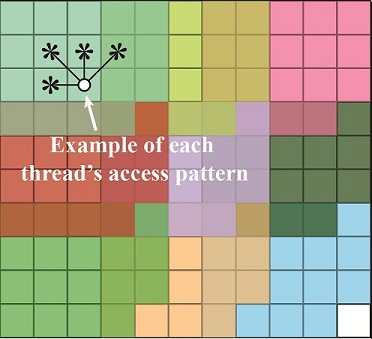
\includegraphics[width=0.48\textwidth]{images/stackedtiles}
\caption{Tiling for Pair-Symmetric Stencil Processing with each tile having a unique color and overlapping tiles have a resultant color that results from mixing colors of overlapping tiles. The pair-symmetric thread access pattern ensures exclusive memory writes.}
\label{fig:Tiling-for-Pair-Symmetric}
\end{figure}

\begin{figure}
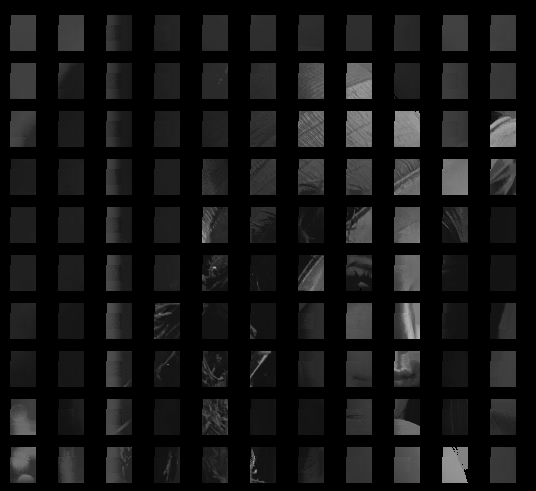
\includegraphics[width=0.48\textwidth]{images/lenatiles}
\caption{Input image after one iteration of pair-symmetric algorithm. Tiles do not have perfect boundaries due to overlaps.}
\label{fig:An-iteration-of}
\end{figure}

If processes were assigned to adjacent tiles, race conditions would occur because the edge cells of the tiles would overlap each other due to intersecting half-width periphery regions, as illustrated in Figure~\ref{fig:Tiling-for-Pair-Symmetric}. To get around this problem, simultaneously processed tiles can be spaced apart in strides such that no two tiles being processed at the same time intersect with one another. An example of such a technique is illustrated in Figure~\ref{fig:An-iteration-of} (the tiles are flipped sideways in this rendering). 

\section{CPU-based Implementation Details}
\label{sec:optimizations} 

\subsection{Memory to computation ratio of Bilateral filtering kernel}
\begin{figure}[h!]
\begin{centering}
\subfigure{ 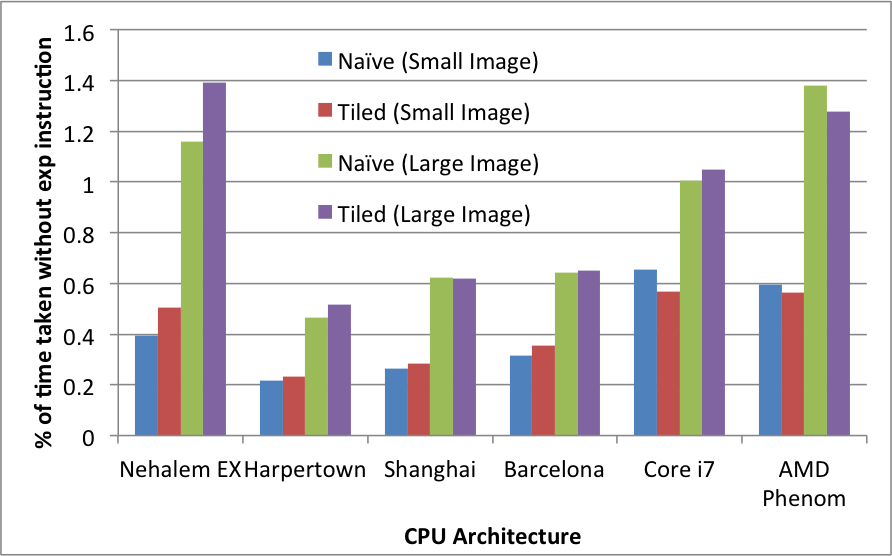
\includegraphics[width=0.48\textwidth]{images/noexplarge}} 
\par\end{centering}
\caption{Percentage of time taken by sequential kernel when run without $exp$ instruction, $filter$ $radius$=10.}
\label{fig:noexp} 
\end{figure}

Unlike traditional regular embarrassingly parallel stencil kernel codes where memory management plays a pivotal role in realizing performance, Bilateral filtering kernel is extremely computationally intensive with only a meager amount of time spent in memory accesses. Bilateral filtering kernel requires computation of $exponential$ function ($exp$ function) which is a major component of time spent in processing. Figure~\ref{fig:noexp} shows the percentage of time taken by Naive Bilateral filtering algorithm\cite{Tomasi1998} and an improved algorithm employing tiled-memory-access pattern on different platforms for a 512x512 pixels small image and a 3000x3000 pixels large image after the $exp$ function was commented out from the computation. The only purpose of this experiment is to justify the fact that traditional memory-access-pattern related optimizations can not improve the performance of Bilateral filtering kernel.

It can be seen that after taking the $exp$ instruction out of the computation, the total sequential execution time is consistently less than 2\% of the original execution time with $exp$ instruction in place. For the smaller image it is strictly less than 1\% of the original time with $exp$ instruction in place. To be precise it is 1.39\% maximum on Intel Nehalem for the larger image and 0.65\% for the smaller image on Core i7 processor. The lower memory transfer time for smaller image is due to the fact that the smaller image fits into the cache memory entirely and hence there are no repeated data transfers between the processor and the main memory.

Since the $exp$ instruction does not involve transfer of data from main memory, it follows from this experiment that memory reuse and memory access pattern related optimizations are not of much help to speed up Bilateral filtering kernel. What Amdahl's law claims, for inherently sequential portion of a parallel algorithm, can be applied here. \\ \textit{The total speedup achieved by optimizations that deal with memory management is limited by the amount of time spent in memory transfers}. Therefore, in this case, traditional optimizations such as tiling/blocking, cache efficient initializations, prefetching, and other NUMA optimizations can only result in a speed up of at most 2\% and hence we have concentrated on optimizations that deal with the complexities of computational aspects of Bilateral filtering kernel.

\subsection{SIMD optimizations}
\label{sub:SIMD1} 
$Intel$'s Streaming SIMD Extension (SSE) is a technique to exploit micro-level parallelism in x86 based processors using SIMD capabilities. SSE can be ideal for tasks that involve repetitive computation such as the 3D heat equation or any other stencil kernels such as Jacobi iterations\cite{kdatta2008}. The matrix multiplication kernel was implemented in \cite{matrix-multi,MatrixMultiFloating} for matrices with integers and floating point numbers. SSE instructions have also been used for image or template matching algorithms such as normalized cross correlation (``NCC'') \cite{NCCmatching}.

Modern day CPUs use SSE that is an extension of MMX technology and is fundamentally similar to MMX. It has 8, 128-bit registers named XMM0 through XMM7. SSE instructions can operate in parallel on data packed in these registers thus providing a theoretically maximum speedup of 16 when working with 1 Byte data structures or 8 when working with 2 Bytes long data structures and so on. There are other extensions of SSE such as SSE2, SSE3, and SSE4.2. Moreover, recent extension of SSE, named Advanced Vector Extensions (``AVX''), uses 256-bit data registers and thus a theoretical peak speedup of 32 is possible.

Our CPU based implementation of Bilateral filtering algorithm explores the use of special purpose registers using both assembly level programming and SSE intrinsics. The advantage of using assembly language is that a programmer can have explicit control of underlying hardware. However, programmer productivity is affected and an in-depth knowledge of underlying hardware is essential. 

Although SSE intrinsics are wrappers for assembly language, it is preferred to use SSE intrinsics due to ease of coding and also due to efficient utilization of available assembly level instructions without knowing the low level details of underlying architecture. A programmer, working with intrinsics, can specify the intrinsic and the appropriate instruction will automatically replace this intrinsic during compilation. Moreover, there are some operations for which there are no assembly instructions and hence in case of assembly level programming the code size can grow to such an extent that readability gets compromised.  

Although the modern compilers usually try to improve the performance by automatically vectorizing, unrolling loops, prefetching, and SIMDization, we were still able to get significant performance improvements alongside compiler optimizations.

\subsection{Reduction Methods}

\label{sub:reduction} Sum by reduction is a technique to compute sum of multiple elements usually stored in contiguous memory locations. There are assembly instructions that can add horizontally packed, single precision, floating point numbers. We used $haddps$ assembly instruction that takes two (source and destination) 128 bit operands, and adds the single precision floating point numbers stored in first and second $dword$ of destination and source operand and stores it in first and third $dword$ of the destination operand respectively. Similarly, the third and fourth $dword$ of destination and source operand are added and stored in second and fourth $dword$ of the destination operand respectively. Both source and destination values must be stored in MMX registers. The SSE intrinsic to perform horizontal add is $\_mm\_hadd\_ps$. It takes two 128 bit operands, each of which is treated as four 32-bit floating point elements. The result of this operation on operand X(X0, X1, X2, X3) and Y(Y0, Y1, Y2, Y3) is (Y3 + Y2, Y1 + Y0, X3 + X2, X1 + X0).

\section{Experimental Testbed}
\label{sec:expt}

\begin{table*}[t]
\begin{tabular}{|l|p{1.2cm}|p{0.8cm}|p{0.8cm}|p{0.8cm}|p{3.5cm}|l|p{2cm}|l|p{0.9cm}|}
\hline 
\textbf{Model}  & \textbf{Clock frequency}  & \textbf{cores per chip}  & \textbf{chips per node}  & \textbf{cores per node}  & \textbf{SIMD support}  & \textbf{Cache/Memory}  & Compiler\\
\hline 
Intel Xeon E5410  & 2.33 $GH_z$  & 4  & 2  & 8  & SSE, SSE2  & 12 MB  & icpc 11.1\\
\hline 
Intel Xeon X7560  & 2.27 $GH_z$  & 32  & 1  & 32  & SSE, SSE2  & 24 MB & icpc 11.1\\
\hline 
Intel Core i7-870  & 2.93 $GH_z$  & 4  & 1  & 4  & SSE, SSE2, SSE3, SSE4.2  & 8MB & icpc 12.0.2\\
\hline 
AMD Opteron 2376  & 2.3 $GH_z$  & 4  & 2  & 8  & SSE, SSE2  & 6MB  & icpc 11.1\\
\hline 
AMD Opteron 8350  & 2.0 $GH_z$  & 4  & 4  & 16  & SSE, SSE2  & 2MB  & icpc 11.1 \\
\hline 
AMD Phenom II X6 1045T  & 2.7 $GH_z$  & 3  & 1  & 6  & SSE, SSE2, SSE4a  & 6MB  & icpc 12.0.2 \\
\hline 
NVidia GeForce GTX 280 & 1296 MHz & 240 & 1 & 240 & - & 1 GB GDDR3 & CUDA 2.0\\
\hline
\end{tabular}\caption{Architectural details of multicore chips employed for experiments}
\label{tab:archs} 
\end{table*}

In order to evaluate our implementation we have tried it on a range of multicore and manycore chips. Table \ref{tab:archs} summarizes architectural details of systems we used during our experiments. 


\subsection{Hardware}
\label{subsec:hw} 
\subsubsection{Intel Xeon}
\label{ss:xeon} We have used two different Xeon chips, E5410 (Harpertown) and X7560 (Nehalem EX). Harpertown is a dual-socket, dual-processor relatively old system with a clock frequency of 2.33 $GH_z$.  Harpertown does not have Intel's hyperthreading (HT) technology which means the maximum number of threads is equal to the number of cores available. Intel Nehalem EX is considerably newer chip having eight-cores processing at a clock frequency of 2.27 $GH_z$. We had access to a Linux cluster from Intel's Manycore Testing Lab (MTL) containing four sockets of Nehalem EX chips thereby making 32 cores available to experiment with. The processors are connected to each other via Intel QPI (Quickpath interconnect) links that can transfer data at 6.4 GT/s. Both of these machines support 64 bit instructions. 

\subsubsection{AMD Opteron}
\label{ss:opteron} AMD Opteron 2376 (Shanghai) chip has private L1 and L2 caches of size 128KB (64 D + 64 I) and 512KB respectively per core along with a 6MB cache shared among all of the cores. It has a clock frequency of 2.30 $GH_z$ and it is a quad-core architecture. Our compute node has two of Shanghai chips making it a total of eight cores to be used for experiments. AMD Opteron 8350 (Barcelona) is similar to Shanghai in many aspects but it has a clock frequency of 2.0 $GH_z$ and the shared cache is only 2MB. Our compute node contains 4 of Barcelona chips and thus we are able to run 16 threads on this node. 

\subsubsection{Intel Core i7}

\label{ss:corei7}Intel Core i7 - 870 supports SSE 4.2 and has AVX technology. The clock frequency is an impressive 2.93 $GH_z$ and it can operate at a maximum of 3.6 $GH_z$ supported by $Intel$'s power boost technology. Its architecture supports hyperthreading which lets an application to execute 8 threads in total; however, we only used one thread per core. It contains 2 memory channels that provide a theoretical maximum memory bandwidth of 21 GB/s. 

\subsubsection{AMD Phenom II}
\label{ss:phenom} AMD Phenom is a six core processor with each core capable of operating at 2.7 $GH_z$. If only three cores are in operation it can run at a maximum of 3.2 $GH_z$. It boasts 128 KB (64 D + 64 I) L1 cache, and 512 KB L2 cache per core in addition to a 6MB L3 cache shared among all six cores. The cache latencies are 3, 13, and 47 clock cycles for L1, L2, and L3 caches respectively. The cache line size is 64 bytes, L1 caches are 2 way set associative, L2 caches are 16-way set associative and L3 cache is 48-way set associative. 

\subsubsection{NVidia GeForce GTX 280}

GTX 280 by NVidia is a GPU chip with 240 CUDA cores with 602 $MH_z$ graphics clock and 1296 $MH_z$ processor clock. GTX 280 is equipped with a 1 GB standard memory with 1107 $MH_z$ memory clock and 141.7 GB/s memory bandwidth. GTX 280 boasts a memory interface width of 512-bit with texture fill rate of 48.2 billion/second. 

\subsection{Software Framework}

\label{subsec:sw} Our implementation for multicores is written in $C++$ and uses OpenMP for parallelization; the GPU implementation uses CUDA. To enrich supported image formats, we use $CImg$ library. 
\subsubsection{Algorithm variations on multicore architectures}
We have implemented a number of variations of Bilateral filtering kernel for multicore chips, results of which are reported in section \ref{sec:results}. Our GPU implementation uses naive algorithm and the pair symmetric algorithm. For multicore chips we have created multiple variations of naive algorithm. These algorithms are labeled as follows: 
\begin{itemize}
\item $BL\_Naive$ is the sequential version of the code, as described by Tomasi\cite{Tomasi1998}. 
\item $BL\_Tiles$ is an improved version of Bilateral filtering kernel that employs data blocking to leverage the availability of multi-level cache hierarchy in the modern multicore CPUs.   
\item $BL\_Assembly$ is the version of Bilateral filtering kernel implemented using assembly level code. 
\item $BL\_A\_Reduction$ is the version of Bilateral filtering that uses assembly language as well as reduction optimizations. 
\item $BL\_Intrinsic$ version uses SSE intrinsics instead of assembly language.
\item $BL\_I\_Reduction$ is the extended version of $BL\_Intrinsic$ that uses the intrinsics that can compute sum of two 128 bit operands in parallel by exploiting the vector array processing. 
\end{itemize}
$BL\_Naive$ has a redundant calculation inside the innermost loop which has been moved out of loop for all other versions. The original instruction involving this calculation looks like
 $$gaussian\_ph = exp\left( \frac{-pd} {2 * sigma\_ph*sigma\_ph}\right);$$
After moving the redundant calculation out of the loop the same instruction becomes
 $$gaussian\_ph = exp( pd * pre\_calc\_sigma\_sq );$$ 
 
Our Bilateral filtering code is open-source licensed under GPL and available from $Google~Code$ repository \url{http://code.google.com/p/blfilter} through SVN version management system. 
\subsubsection{Input Image}
In order to analyze the behavior of our kernel with varying image sizes, we have executed our kernel with two different images. One that fits into cache easily and the other that does not fit into cache but fits into main memory. Both of the images were converted to single spectrum images represented by single precision numbers for each pixel. The smaller image was 512 pixels wide and 512 pixels high, thus requiring 1MB memory to store it. As shown in Table~\ref{tab:archs} all of the multicore systems have cache memories bigger than 1 MB. The second image was 3000 pixels wide and 3000 pixels high and hence requires little more than 34 MB of memory to store it. None of the multicore cache memories were big enough to store this image entirely.

\section{Performance Results}
\label{sec:results}
\subsection{Performance of Bilateral filtering kernel on CPU}
For all of our experiments the filter radius was kept at 10, subsequently making the filter Window of size 21 x 21. The spatial spread and the photometric spread were also set to 10. The optimization flag $O3$ was used for all experiments in addition to SSE2 for SIMDization. For Core i7 chip compiler flag SSE4.2 was used instead of SSE2. We do not use hyperthreading, i.e., there are no more than one thread per core. 

\begin{figure*}[t!] 
\begin{centering} 
\subfigure[Nehalem-EX Xeon X7650]{ \includegraphics[width=0.3\textwidth]{images/nehalem} \label{fig:Nehalem} } 
\subfigure[Harpertown Xeon E5410]{ 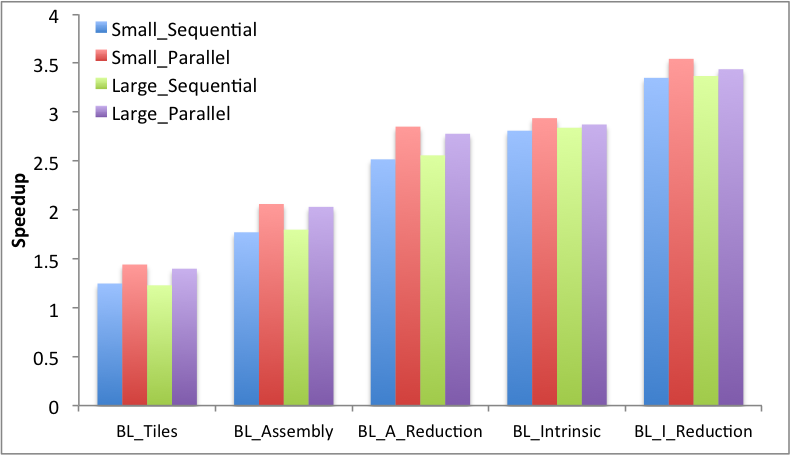
\includegraphics[width=0.3\textwidth]{images/harpertown} \label{fig:harpertown} } 
\subfigure[Core i7 - 870]{ 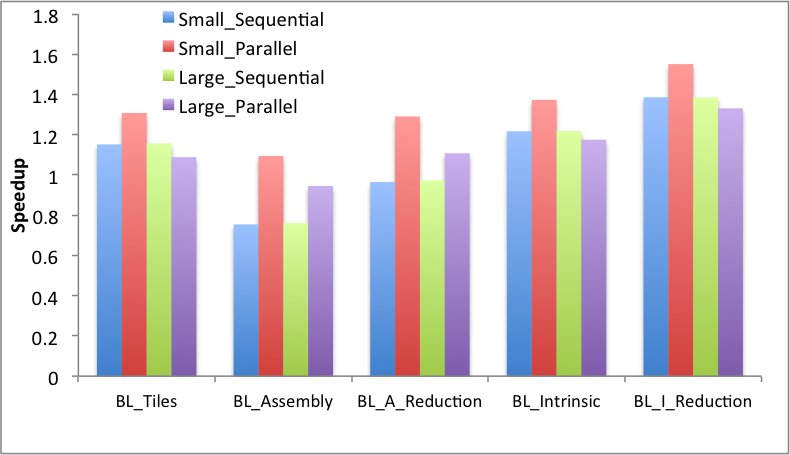
\includegraphics[width=0.3\textwidth]{images/corei7} \label{fig:corei7} } 
\end{centering}
\caption{Bilateral filtering kernel on Intel chips. The baseline version is BL\_Naive version, auto optimized by compiler with O3 and SSE flags.} 
\label{fig:comparisonIntel} 
\end{figure*} 

\begin{figure*} 
\begin{centering} 
\subfigure[Barcelona AMD Opteron 8350]{ 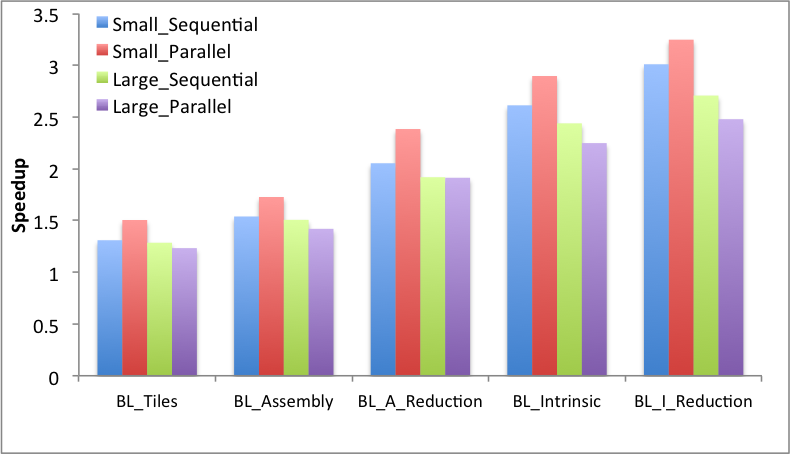
\includegraphics[width=0.3\textwidth]{images/barcelona} \label{fig:barcelona} } 
\subfigure[Shanghai AMD Opteron 2376]{ \includegraphics[width=0.3\textwidth]{images/shanghai} \label{fig:Shanghai} } 
\subfigure[AMD Phenom II 1045T]{ 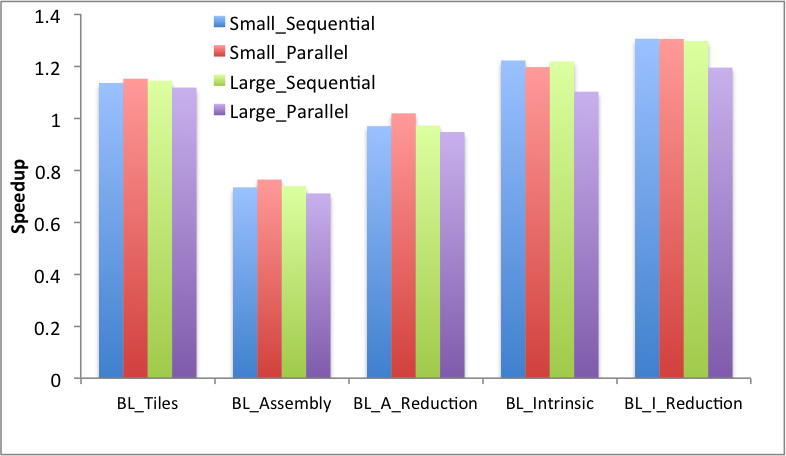
\includegraphics[width=0.3\textwidth]{images/phenom} \label{fig:Phenom} } 
\end{centering}
\caption{Bilateral filtering kernel on AMD chips. The comparison is with BL\_Naive version, auto optimized by compiler with O3 and SSE flags.} 
\label{fig:comparisonAMD} 
\end{figure*} 
\begin{figure*}[t!] 

\begin{centering} 
\subfigure[Harpertown Xeon E5410]{  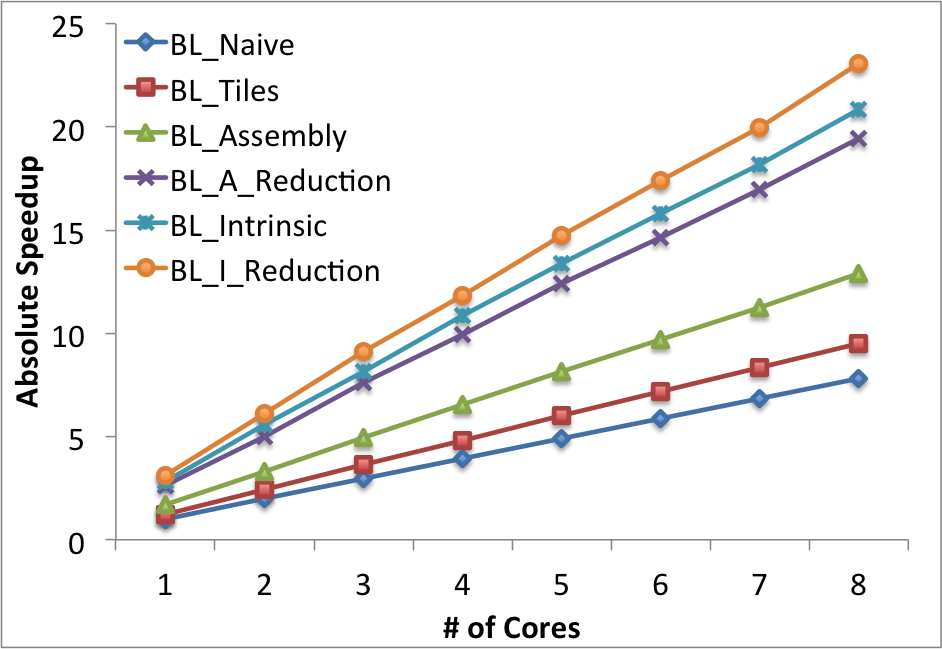
\includegraphics[width=0.32\textwidth]{images/harpertownfinal} \label{fig:harpertownFinal} } 
\subfigure[Core i7 - 870]{ \includegraphics[width=0.32\textwidth]{images/corei7final} \label{fig:corei7Final} } 
\subfigure[Nehalem-EX Xeon X7650]{ \includegraphics[width=0.32\textwidth]{images/nehalemfinal} \label{fig:NehalemFinal} } 
\end{centering}
\caption{Comparison of combined speedup due to SIMDization and OpenMP parallelization on Intel chips for different algorithms} 
\label{fig:comparisonFinalIntel} 
\end{figure*} 

\begin{figure*} 
\begin{centering} 
\subfigure[Barcelona AMD Opteron 8350]{ 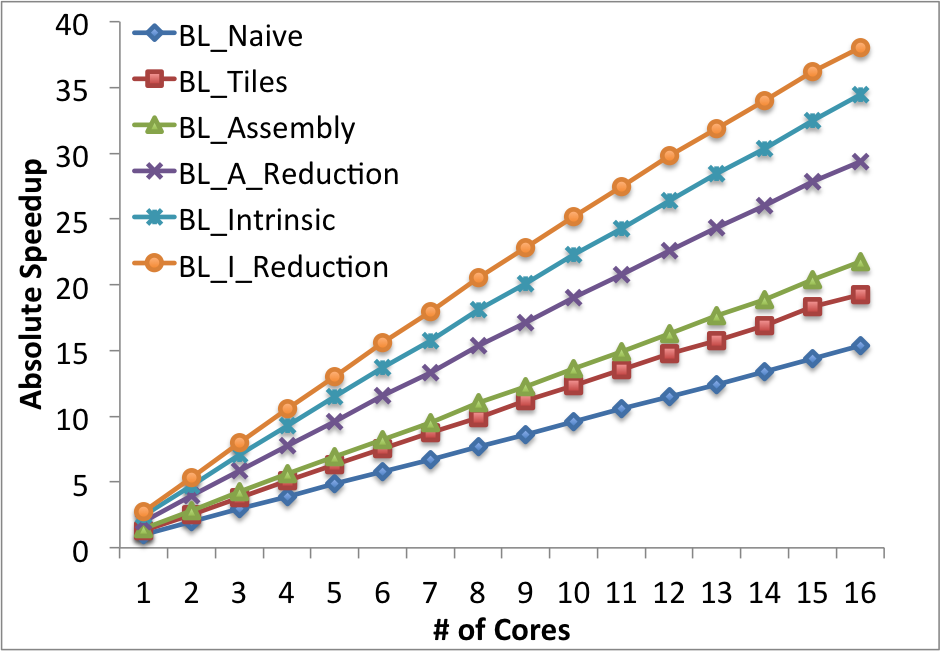
\includegraphics[width=0.3\textwidth]{images/barcelonafinal} \label{fig:barcelonaFinal} } 
\subfigure[Shanghai AMD Opteron 2376]{ 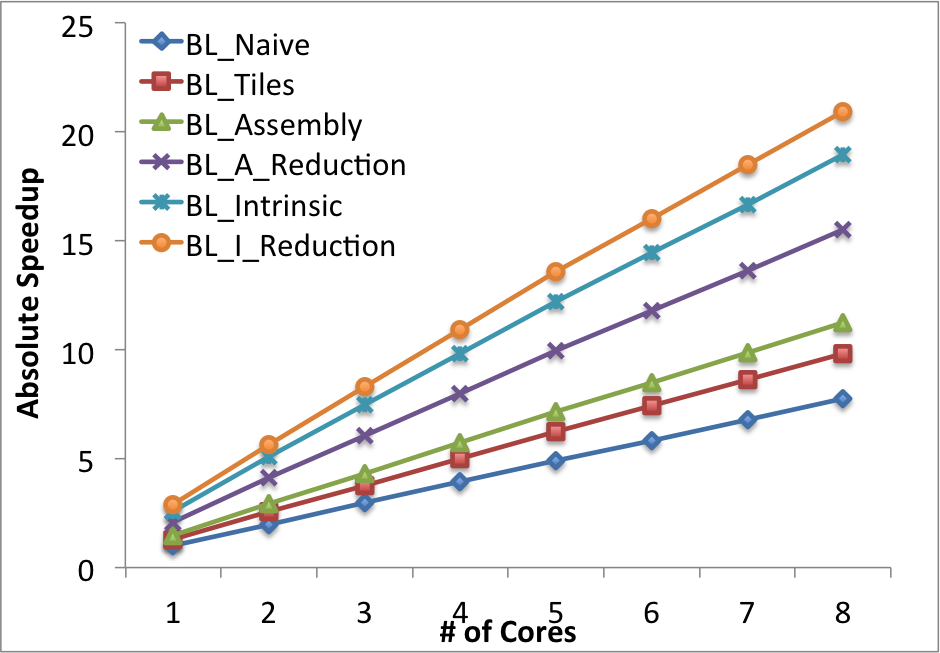
\includegraphics[width=0.3\textwidth]{images/shanghaifinal} \label{fig:ShanghaiFinal} } 
\subfigure[AMD Phenom II 1045T]{ 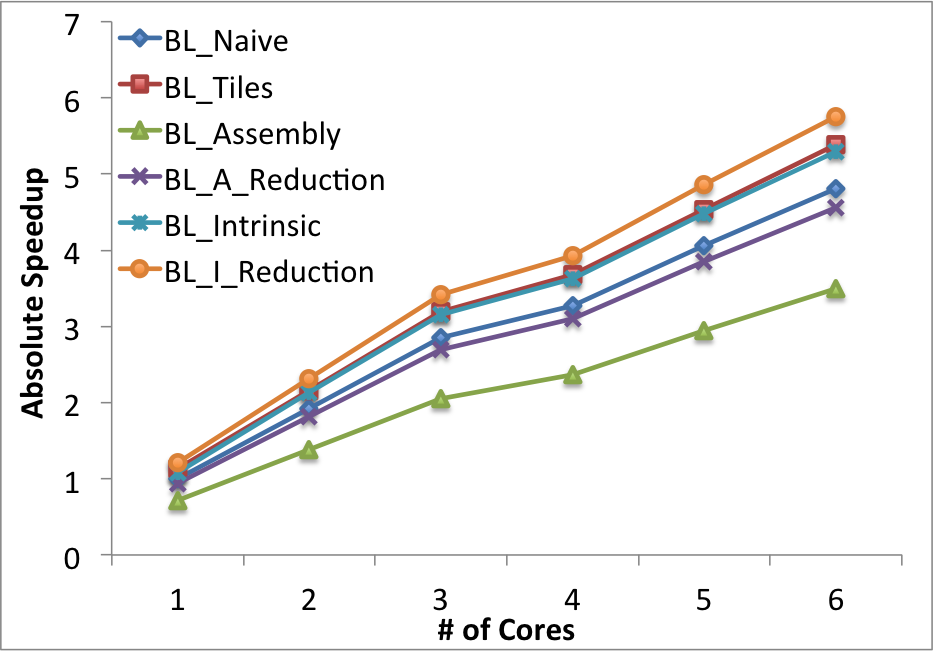
\includegraphics[width=0.3\textwidth]{images/phenomfinal} \label{fig:PhenomFinal} } 
\end{centering}
\caption{Comparison of combined speedup due to SIMDization and OpenMP parallelization on AMD chips for different algorithms.} 
\label{fig:comparisonFinalAMD} 
\end{figure*} 


Figure~\ref{fig:comparisonIntel} compares different algorithms on all three $Intel$ chips. In this experiment we are comparing the absolute speedup achieved by the respective algorithm compared to BL\_Naive algorithm. It is important to note that these results are for micro level parallelism (use of 128 bit special purpose registers) only and do not consider speedup due to high level (OpenMP) parallelization. The parallel versions shown here are compared against the parallel version of BL\_Naive algorithm. The speedup for all algorithms is still bounded by the theoretical peak speedup which happens to be four here since we work with 32bit floating point numbers. Interestingly, although we use compiler optimization flags such as -O3 and -xSSE2, i.e., there is automated vectorization taking place in all the algorithms, our hand coded vectorization is superior in many cases.

The speedup shown by BL\_Tiles is mostly due to the computation reduction as discussed in section \ref{subsec:sw} because we do not use special purpose registers in this algorithm. It can be seen from figure~\ref{fig:comparisonIntel} that the parallelism due to SIMDization is limited by four which is the theoretical maximum possible speedup due to SSE registers as discussed in section \ref{sub:SIMD1}.

As seen in figure~\ref{fig:Nehalem}, the maximum speedup achieved on Nehalem architecture only using SSE optimization is 2.29x for the smaller image and 1.33x for the larger image. Smaller image generally performs better because the time to copy data to SSE registers is less as the entire image is always available in the cache memory. The BL\_Naive algorithm outperforms our assembly level implementations but it is slower than our intrinsic based implementations in all cases. The reason for this is that the auto SIMDization by compiler is more efficient than our implementation for Nehalem architecture. Intel Harpertown, which is a relatively older chip, shows an impressive speedup of 3.54x (Figure~\ref{fig:harpertown}) even though compiler optimizations are still in place. 

Another interesting observation is the results on Intel Core i7 architecture shown in Figure~\ref{fig:corei7}, where we have the absolute speedup of less than $1$. This indicates the fact that the automated compiler optimizations on newer chips are superior than on older chips. These experiments were run with $SSE4.2$ compiler flag and hence the compiler is able to exploit SIMDization automatically thus making it difficult to surpass it using assembly level coding. 

However, our algorithms that use SSE intrinsics and reduction, i.e. BL\_A\_Reduction, BL\_Intrinsic, and BL\_I\_Reduction are able to provide better speedups than those achieved by compiler optimizations as shown in Figure~\ref{fig:comparisonIntel} and Figure~\ref{fig:comparisonAMD}.

Figure~\ref{fig:comparisonAMD} shows the similar comparison across AMD chips. The results are in tune with those for Intel platform. As shown in Figure~\ref{fig:barcelona} for Barcelona, which is a relatively older chip, the maximum speedup is 3.24x for BL\_I\_Reduction algorithm. Similarly, for AMD Shanghai, as shown in Figure~\ref{fig:Shanghai}, the maximum speedup achieved by exploiting SIMDization is 3.02x for BL\_I\_Reduction algorithm. The case of AMD Phenom is shown in Figure~\ref{fig:Phenom}. The auto tuning applied by the compiler outperforms the manual tuning in case of BL\_Assembly and BL\_A\_Reduction. However, BL\_Intrinsic and BL\_I\_Reduction are still able to outperform compiler optimizations. The maximum speedup achieved in this case is 1.30x.

The next set of results demonstrate the total speedup due to OpenMP as well as due to SIMDization. It is interesting to see how speedup due to OpenMP multiplies with the speedup due to SSE optimizations to exhibit super linear speedup.

Figure~\ref{fig:harpertownFinal} shows the performance of Bilateral filtering kernel on Intel Harpertown. This machine has 8 cores and the maximum combined speedup achieved is 20.91x. The speedup achieved only using only SSE optimization was 2.69x and the speedup achieved by BL\_Naive algorithm using 8 cores is 7.73x.

Intel Nehalem chip with 32 cores does not show a super-linear speedup as shown in Figure~\ref{fig:NehalemFinal}. However, the reason behind this is the lack of enough parallelism that can be afforded by the kernel for this image. Both optimizations still multiply their individual speedup to result in the combined speedup. The total combined speedup is 26.46x using 32 cores, the speedup only due to SSE was 1.12x and the speedup for BL\_Naive is 23.47x.

Intel Core i7 chip (Figure~\ref{fig:corei7Final}) also demonstrates the similar behavior. The final speedup of 4.63x, using 4 cores, is a result of speedup due to SSE which is 1.33x and speedup due to OpenMP which is 3.48x. 

Figure~\ref{fig:comparisonFinalAMD} shows a similar comparison over various AMD chips. Figure~\ref{fig:barcelonaFinal} shows the speedup for Barcelona chip. This chip has 16 cores with a combined maximum speedup being 38.03x. The speedup achieved using SSE optimizations was 2.48x and the speedup for BL\_Naive was 15.34x and thus these both realize a speedup of 38.03x using 16 cores.

AMD Shanghai similarly shows an impressive speedup of 20.92x (Figure~\ref{fig:ShanghaiFinal}). The interesting case is with AMD Phenom as shown in Figure~\ref{fig:PhenomFinal}. The speedup drops a little as number of cores increases beyond three. The reason behind this is the turbo core technology as discussed in section (\ref{ss:phenom}). When there are a maximum of three cores being used the clock frequency scales up to 3.6 $GH_z$ but as soon as more threads are created the clock frequency steps down to 2.7 $GH_z$. 

\subsection{Performance of Bilateral filtering kernel on GPU}

We used the NVIDIA GTX 280 for benchmarking the performance of our CUDA implementations. Our implementations' variable parameters were the image size, the filter window size, and the grid dimensions (\# blocks horizontal * \# of blocks vertical concurrently executed) and block dimensions (\# of threads horizontal * \# of threads vertical in each block). The tests used two images: a large image with 3000 x 3000 pixels and a small image with 768 x 512 pixels.

On the GPU, our pair-symmetric algorithm outperformed our naive algorithm for every set of tests. For example, Figure~\ref{fig:hw10} shows the pair-symmetric algorithm's best timing to be roughly 75\% of the naive algorithm's best timing for processing a 3000 x 3000 image using a 21 x 21 pixel filter window. The test that gave the closest difference in timing as shown in Figure~\ref{fig:hw10light} was processing a 768 x 712 pixel image using a 11 x 11 window size. In this test, the pair-symmetric algorithm's best timing was at a virtual tie with the naive algorithm's best timing at 0.00390 seconds, but upon further testing we found the pair-symmetric algorithm's optimal timing to be 0.00388 seconds when changing the grid dimension to 16 x 16 concurrent blocks, thus slightly outperforming the naive algorithm. Figures \ref{fig:hw10} and \ref{fig:hw10light} show exponential rises in execution time for both algorithms as block vertical dimension decreased. Due to runtime complexity of the bilateral filter being the square of the filter width, Figures (b) and (d), which reflect tests that used a 5 pixel filter width, do not exhibit the steep curvature that Figures (a) and (c) exhibit.

While our tests returned a maximum 25\% reduction in execution time, our pair-symmetric algorithm has the potential to reach a near 50\% reduction in execution time. Furthermore, the benchmarks of our pair-symmetric algorithm reveal minor irregularities in the trajectory of performance derived from execution timings versus respective incremental adjustments of parameter values such as CUDA block and grid dimensions. The main cause of both of these observations is shared memory. To better understand the impact of the additional shared memory transactions that our pair-symmetric algorithm requires, whereas the naive algorithm does not require shared memory for output storage, we implemented a single-threaded CPU-based version of both the naive bilateral filter algorithm and pair-symmetric algorithm so that native-memory (RAM, L1, or L2 cache) could substitute for the GPU's shared memory. The results were remarkably illustrative of our pair-symmetric algorithm's potential. The naive algorithm running on the CPU with a filter width of 10 pixels processed a 3000 x 3000 image in an average of 1206.7 seconds while our pair-symmetric algorithm took 611.8 seconds - a 49.23\% reduction in execution time. Moreover, when replacing shared memory transactions with dummy register transactions in our CUDA implementation of the pair-symmetric algorithm, we observed a consistent 40\% reduction in execution time. From these findings, we conclude that the inferior speed of GPU shared memory transactions to register transactions is what limited our pair-symmetric algorithm's performance gains to  a maximum of 33\%, i.e., achieving timings no less than 75\% of the naive algorithm's timings. To further verify this inference, we meticulously stepped through the Parallel Thread Execution (PTX) code - CUDA's quasi-assembly language - of our CUDA implementations to ensure that no unintended optimizations were being made by the compiler when substituting shared memory transactions with dummy register transactions. Not only were no optimizations being made but the PTX code showed that the shared memory transactions required additional load and store instructions, further evidencing the cost of using shared memory.

Another challenge in interpreting our results was porting the concept of "speed-up" to general purpose GPU programming. Since speed-up is necessarily with respect to a reference timing, we used the same reference timing that our CPU optimizations used---that is how we calculated the 235.5x speed-up figure stated in the abstract of this paper---and we also made another reference timing by running our GPU implementations using a single thread. For example, using a single thread operating with filter width of 10 pixels to process a 768 x 512 pixel image, the time taken for the GTX280 to complete this execution was an average of 177.9 seconds for both of our algorithms; using a filter width of 5 pixels, the average execution time was 50.5 seconds for both algorithms. With respect to these reference timings, the speed-up is roughly 20,500x for the 10 pixel filter width and 12,440x for the 5 pixel filter width.

\begin{figure}[t!] 
\begin{centering} 
\subfigure[Large Image, Filter Width = $10$]{ 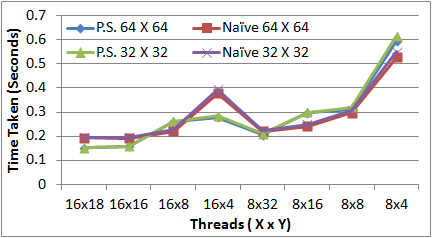
\includegraphics[width=0.4\textwidth]{images/gpuhw10} \label{fig:hw10} } 
\subfigure[Large Image, Filter Width = $5$]{ 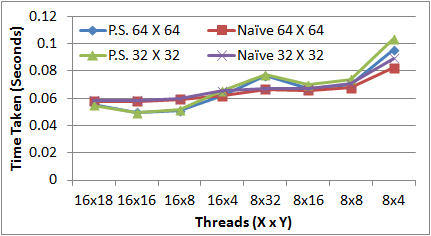
\includegraphics[width=0.4\textwidth]{images/gpuhw5} \label{fig:hw5} } 
\subfigure[Smaller Image, Filter Width = $10$]{ 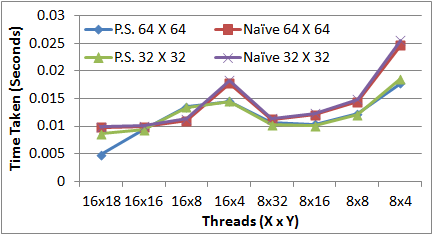
\includegraphics[width=0.4\textwidth]{images/gpuhw10light} \label{fig:hw10light} } 
\subfigure[Smaller Image, Filter Width = $5$]{ 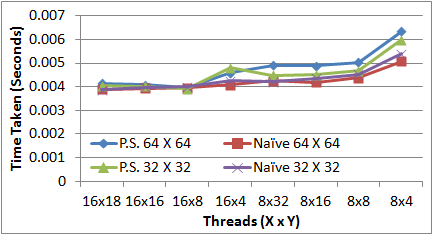
\includegraphics[width=0.4\textwidth]{images/gpuhw5light} \label{fig:hw5light} } 
\end{centering}
\caption{Performance of Naive and pair-symmetric (P.S.) Bilateral filtering kernel algorithms on GTX 280 NVidia card for both smaller image and larger image.} 
\label{fig:gpuresults} 
\end{figure} 

\section{Conclusion and future work}
\label{sec:conclusion} 
Modern day scientific applications demand higher computational capabilities than before and performance gains are no longer driven by clock speed. Chip manufacturers are trying to meet this demand by adding multiple cores on a chip equipped with multiple levels of cache hierarchy and enhanced SIMD extensions. In this paper we have tried to optimize Bilateral filtering kernel using both high level and low level parallelism. Our interest is to develop an efficient parallelization method for modern multicore architectures that can be applied to any spatially invariant and inseparable filter kernel and potentially to any compute-intensive regular numeric application. We have also documented why traditional optimization methods for multicores are not as effective for Bilateral filtering kernel compared to memory intensive kernels. It can be seen from Figure~\ref{fig:comparisonIntel}, and Figure~\ref{fig:comparisonAMD} that a stencil kernel could be optimized by using SSE intrinsics even though the compiler optimizations are in place. Moreover, the reduction methods can provide a decent speedup where applicable. These findings will guide the auto optimizers and auto tuners to include SSE intrinsics as an essential optimization approach.


\bibliographystyle{IEEEtran} \bibliography{paper} \end{document} 
